\section{Other claims}

\subsection{Counterexamples for straightforward attempts}

\subsubsection*{Avoiding the same pattern is not enough.} 
\label{sec:bad-example0}

It might be tempting to conjecture that if $X$ avoids $P$, then the \greedy touch matrix $\Greedy(X)$ avoids $P$ as well ($P$ refers both to a permutation pattern and its matrix representation). While this holds for the simple case $P=(2,3,1)$ in the ``no initial tree''-case (proof left as an exercise for the reader), in general it is not true. Figure~\ref{fig:pattern-counter} shows a counterexample ($P = (3,2,1)$).

\begin{figure}[h]
\centering
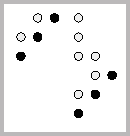
\includegraphics[scale=1.2]{counter1.pdf}
\caption{Access points are black circles, points touched by \greedy are gray circles. Input avoids (3,2,1), but output contains (3,2,1).}
\label{fig:pattern-counter}
\end{figure}

\subsubsection*{\greedy is not decomposable.}
\label{sec:bad-example1}

One could prove a decomposition theorem similar to Theorem~\ref{lem: main} for \greedy, if \greedy were \emph{decomposable}.
By this we mean that for a $k$-decomposable input sequence, considering a certain level $P=\tilde{P}[P_1,\dots,P_k]$ of the decomposition tree, \greedy touches a region $R(i,j)$, iff the corresponding point $(i,j)$ is touched by \greedy, when executed on the contracted instance $\tilde{P}$. Alas, this property does not hold for \greedy, as shown on Figure~\ref{fig:decomp-counter}.

\begin{figure}[h]
\centering
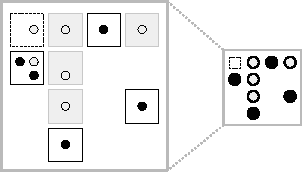
\includegraphics[scale=1.3]{counter2.pdf}
\caption{Access points are black circles, points touched by \greedy are gray circles. Left: block decomposition of input, and \greedy execution. Top left region is touched. Right: \greedy execution on contracted instance. Top left point not touched.}
\label{fig:decomp-counter}
\end{figure}

\subsubsection*{No permutation input-revealing gadget with initial trees.}
\label{sec:bad-example2}

A permutation input-revealing gadget for \greedy would allow us to strengthen the bound in Theorem~\ref{thm:pattern-avoidance} from quasilinear to linear. In Figure~\ref{fig:gadget-counter} we sketch a construction that shows that such a gadget can not exist, if initial tree is allowed, even if the input is the preorder sequence of a path.


\begin{figure}[h]
\centering
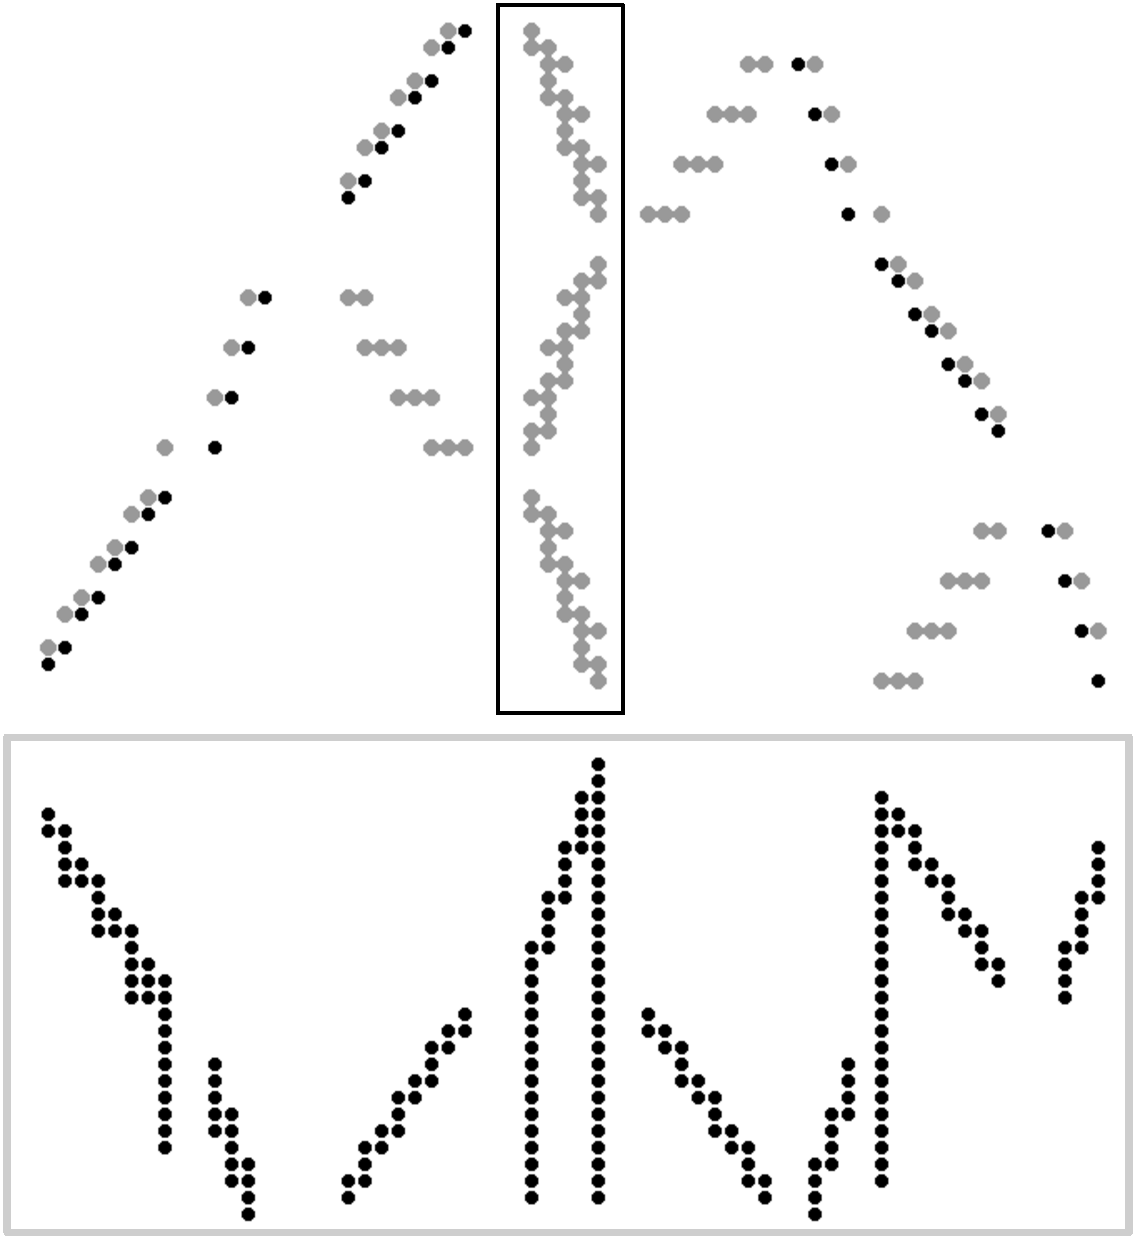
\includegraphics[scale=0.7]{nogadget.pdf}
\caption{A \greedy execution with initial tree. Access points and initial tree are shown with black circles, points touched by \greedy are gray circles. Black rectangle marks a region in which all permutations are contained, but there is no access point inside. Gray rectangle marks initial tree.}
\label{fig:gadget-counter}
\end{figure}

\subsection{Tightness of $O(n \log k)$ for $k$-decomposable permutations}
\label{sec:tight-block} 
In this section, we show that the upper bound of $\opt(X) = O(n \log k)$ for $k$-decomposable permutations is tight, by arguing that there is a sequence that matches this bound. 
We will use the following claim, which is proved in \S\,\ref{lem:decomp opt lower-bound}, and restated here. 

\begin{lemma} 
Let $X$ be any input sequence and $\tset$ be its tree decomposition. Then 
\[\opt(X) \geq \sum_{P \in \tset} \opt(P) -  2n\]
\end{lemma} 

Let $P'$ be a sequence of size $k$ where $\opt(P') = \Omega(k \log k)$. 
Then we construct the tree $\tset$ which is a complete degree-$k$ tree of depth $d$, with each node $v \in \tset$ having the template $P_v = P'$.  
Then $n = k^d$, and each non-leaf node $v \in N(\tset)$ has $\opt(P_v) = \Omega(k \log k)$.  
There are $k^{d-1} = n/k$ non-leaf nodes, so we have $\opt(X) \geq \Omega(k \log k) \cdot \frac{n}{k} = \Omega(n \log k)$. 


\subsection{Decomposition of $k$-increasing sequences}
\label{sec:decomposition_monotone}

Given a permutation $X = (X_1, \dots,X_n)$, a subsequence of $X$ of size $k$ is a sequence $(X_{i_1}, \dots, X_{i_k})$, where $1 \leq i_1 < \cdots < i_k \leq n$.

\begin{lemma}
\label{lem:decomposition_monotone}
Let $X \in S_n$ be an arbitrary permutation. The following statements are equivalent:
\begin{compactenum}[(i)] 
\item $X$ is $(k,\dots,1)$-free,
\item There exist pairwise disjoint subsequences $Y_1, Y_2, \dots, Y_{k-1}$ of $X$, such that $Y_i$ is increasing for all $i=1,\dots,k-1$, and $|Y_1| + \cdots + |Y_{k-1}| = n$.
\end{compactenum}
\end{lemma}
\begin{proof}
(ii) $\implies$ (i):\\
Let $Y_1, \dots, Y_{k-1}$ be increasing subsequences of $X$, as in the statement of the lemma, and suppose there exists a subsequence $X' = (X_{i_1}, \dots, X_{i_k})$ of $X$ order-isomorphic to the pattern $(k,\dots,1)$. Since $X'$ is decreasing, no two elements of $X'$ can be in the same subsequence $Y_i$. This is a contradiction, since we have only $k-1$ subsequences. Therefore, such an $X'$ cannot exist, and $X$ is $(k,\dots,1)$-free.

(i) $\implies$ (ii):\\
Assume that $X$ is $(k, \dots, 1)$-free. We construct the decomposition of $X$ into increasing subsequences $Y_1, \dots, Y_{k-1}$ as follows. We look at the plot of permutation $X$, and we refer interchangeably to elements of $X$ and points in the plot of $X$. Let $Y_1$ be the ``wing'', i.e.\ the points in the plot of $X$ that form an empty rectangle with the top left corner (by this definition, we have $X_1 \in Y_1$). Clearly, $Y_1$ forms an increasing subsequence of $X$. We now remove the elements of $Y_1$ from $X$ and similarly find $Y_2$ as the wing of the remaining points. We repeat the process, thereby finding $Y_1, Y_2, \dots$. We claim that we run out of points before reaching $Y_k$, thus constructing a decomposition of $X$ as required by the lemma.

Suppose otherwise that we have reached $Y_k$, and consider an arbitrary point $X_{i_k} \in Y_k$. Since $X_{i_k}$ was not chosen in $Y_{k-1}$, the rectangle with corners $X_{i_k}$ and the top-left corner has some point from $Y_{k-1}$. Pick such a point, and denote it as $X_{i_{k-1}}$. Observe that $X_{i_{k-1}} > X_{i_k}$, and $i_{k-1} < i_k$. Since $X_{i_{k-1}}$ was not chosen in $Y_{k-2}$, we can pick a suitable $X_{i_{k-2}}$ in $Y_{k-2}$. Continuing in this fashion, we construct the subsequence $X_{i_1},...,X_{i_k}$ of $X$ that forms the forbidden pattern $(k,\dots,1)$, a contradiction.
\end{proof}

\subsection{Comparing easy sequences}
\label{sec:comparisons}

\subsubsection*{Easy sequences not captured by any known bounds.}
\label{sec:easy-examples}
We show a sequence $X$ where $UB(X) = \Omega(n \log n)$, $k(X) = \sqrt{n}$, and $\opt(X) = O(n)$. By $UB$ we denote the ``unified bound''~\cite{unified} that subsumes both the working set, dynamic finger and entropy bounds. At this time, however, $UB$ is not known to be matched by any online BST. $UB$ can be seen as the sum of logs of ``$L_1$ distances''. In other words, $X$ is an easy sequence that is not captured by the known classes of easy sequences studied in the literature.  

Consider a point set $\pset$ that is the perturbation of the $\sqrt{n}$-by-$\sqrt{n}$ grid: Let $\ell = \sqrt{n}$, and  
\[\pset = \set{(i \ell + (j-1), j \ell + i-1): i,j \in [\ell] }.\]
Denote the point $(i\ell+(j-1), j \ell +(i-1))$ by $p(i,j)$.  
It is easy to check that there are no two points aligning on $x$ or $y$ coordinates: If $p(i,j)$ agrees with $p(i',j')$ on one coordinate, it implies that $i= i'$ and $j=j'$.   
Therefore, this point set corresponds to a permutation $X \in S_n$. 
Figure~\ref{fig:examples}(i) illustrates the construction. The following lemma shows that $k(X) = \sqrt{n}$. 

\begin{lemma} 
$X$ contains all patterns $\sigma$ of size at most $\ell$. 
\end{lemma} 
\begin{proof} 
Pattern $\sigma$ corresponds to point set $\set{(\sigma_t, t)}_{t=1}^{k}$, this is order-isomorphic to $p(\sigma_1, 1), p(\sigma_2,2),\ldots, p(\sigma_k, k)$.
\end{proof} 


\begin{proposition} 
$UB(X) = \Omega(n \log n)$. 
\end{proposition} 


Finally, we show that $\opt(X) = O(n)$ by describing an offline algorithm that achieves this bound.
Our algorithm is similar to \greedy, where we augment some extra steps.
First, partition $[n]$ into $I_1,\ldots, I_{\ell}$ such that $I_j = \set{(j-1)\ell +1, j \ell}$. 
Notice that the access sequence starts by touching elements $p(1,1) \in I_1,p(2,1) \in I_2, \ldots, p(\ell,1) \in I_{\ell}$ and then back to $p(2,1)\in I_1$ and so on. 
This occurs for $\ell$ rounds.    

The algorithm proceeds just like \greedy, except that, when accessing $p(i,j)$,  after touching the minimal elements, it also touches the two boundaries of the interval $I_i$, i.e. $(i-1) \ell +1$ and $i \ell$.   
  
\begin{proposition} 
The algorithm produces a feasible solution. 
\end{proposition} 


\begin{proposition} 
The cost of this algorithm is $O(n)$. 
\end{proposition} 

A slightly more involved inductive argument shows that \greedy too has linear cost on $X$.

\begin{proposition} 
$\Greedy(X) = O(n)$. 
\end{proposition} 

\subsubsection*{Pattern avoidance and dynamic finger.} 
\label{sec:df-comp}
We show examples that $k(X)$ and the dynamic finger bound (denoted by $DF(X)$) are not comparable. 
Figure~\ref{fig:examples}(ii) illustrates a sequence $X$ where $DF(X) = O(n)$ and $k(X) = \Omega(\sqrt{n}/ \log n)$. 
First, the sequence $X$ starts with the perturbed grid construction of size $f(n)$-by-$f(n)$ where $f(n) = \sqrt{n} /\log n$; then the sequence continues with a sequential access of length $n - f(n)^2$. 
Notice that, in the first phase of the sequence, the distances between consecutive points are $|X_{i+1} - X_i| = O(f(n))$, except for at most $f(n)$ pairs, which have distance $O(f(n)^2)$. 
In the second phase, the distances are one. So $DF(X) = O(f(n)^2) \log f(n) + O(n) = O(n)$. 
On the other hand, the $f(n)$-by-$f(n)$ grid contains all permutations of size $f(n)$, so we have $k(X) = \Omega(\sqrt{n}/ \log n)$.


Figure~\ref{fig:examples}(iii) illustrates a $2$-recursively decomposable sequence (thus having $k(X) = 3$) whose dynamic finger bound is $\Omega(n \log n)$; to see this, notice that $|X_{i+1} - X_i| \geq n/2$ for $i = 1,\ldots, n/2$, so we have $DF(X) \geq \frac{n}{2} \log (n/2)$.   

\iffalse 
\begin{figure}[h]
\centering
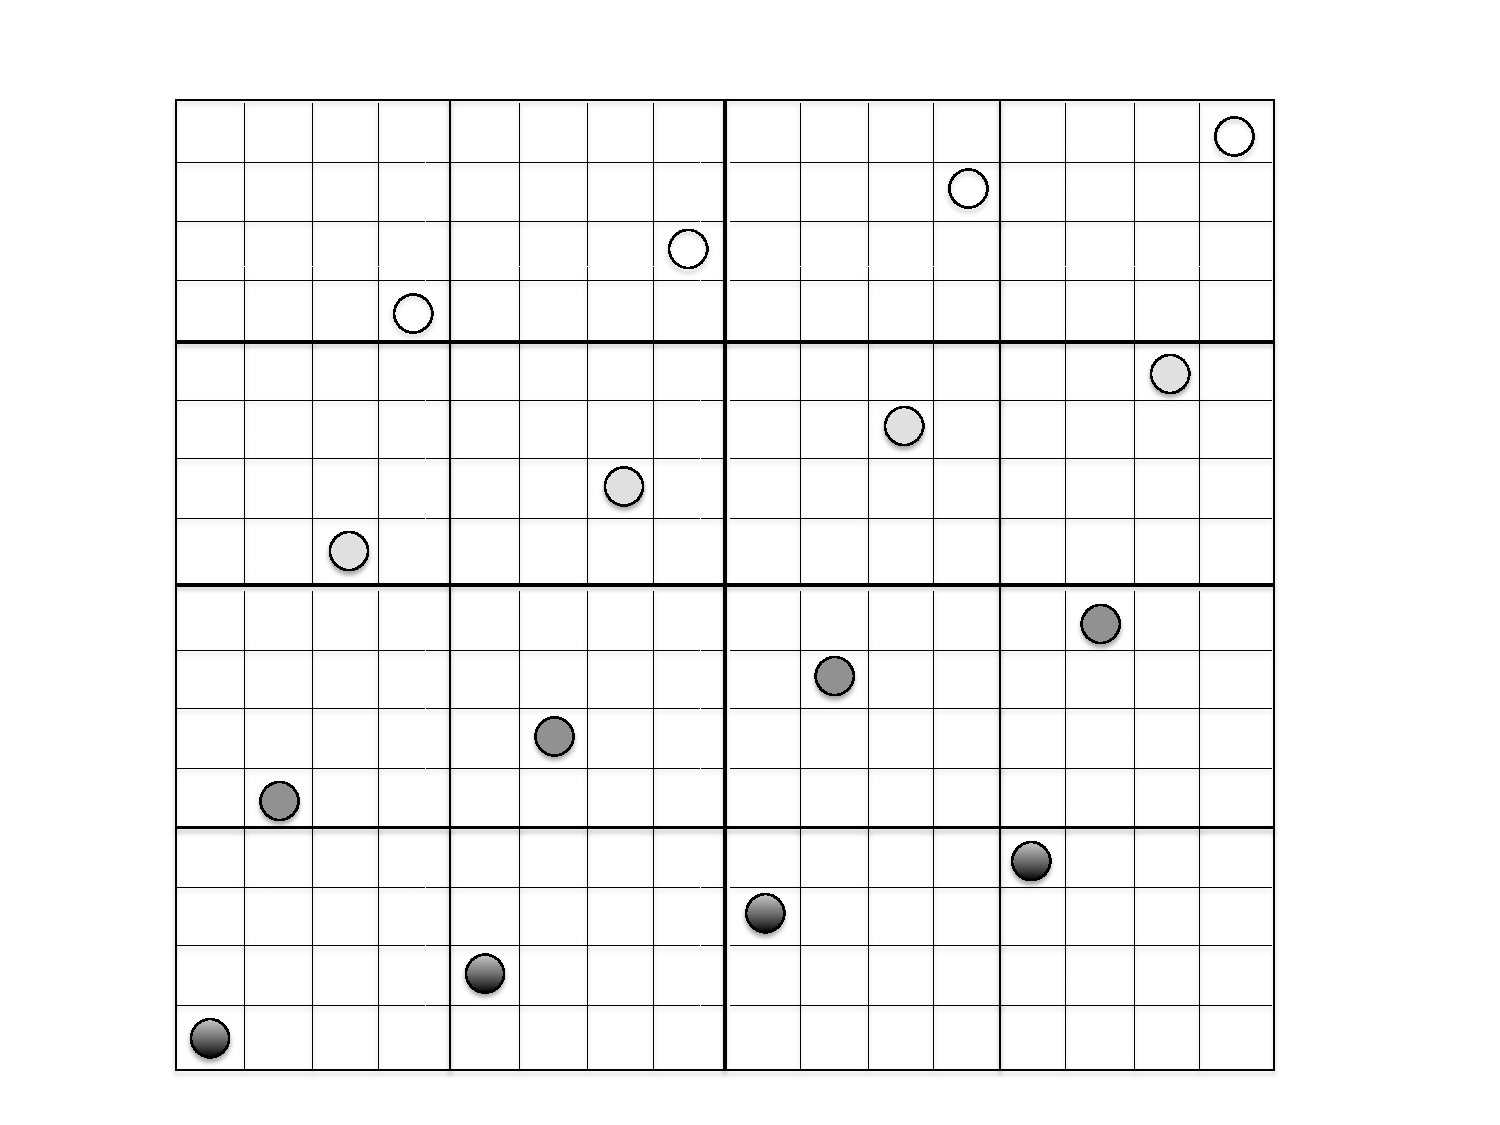
\includegraphics[scale=0.3]{avoiding-linear.pdf}
\label{fig:avoiding-linear}
\caption{An example of the ``perturbed grid'' construction when $\ell=4$.}
\end{figure}
\fi

\subsubsection*{Easy non-decomposable sequence.}
Figure~\ref{fig:examples}(iv) shows the non-decomposable input sequence $X = (n/2, n, 1, n-1, 2, \dots)$ on which \greedy achieves linear cost (to see this, observe that \greedy touches at most three elements in each row).   
 

\begin{figure}[h]
\centering
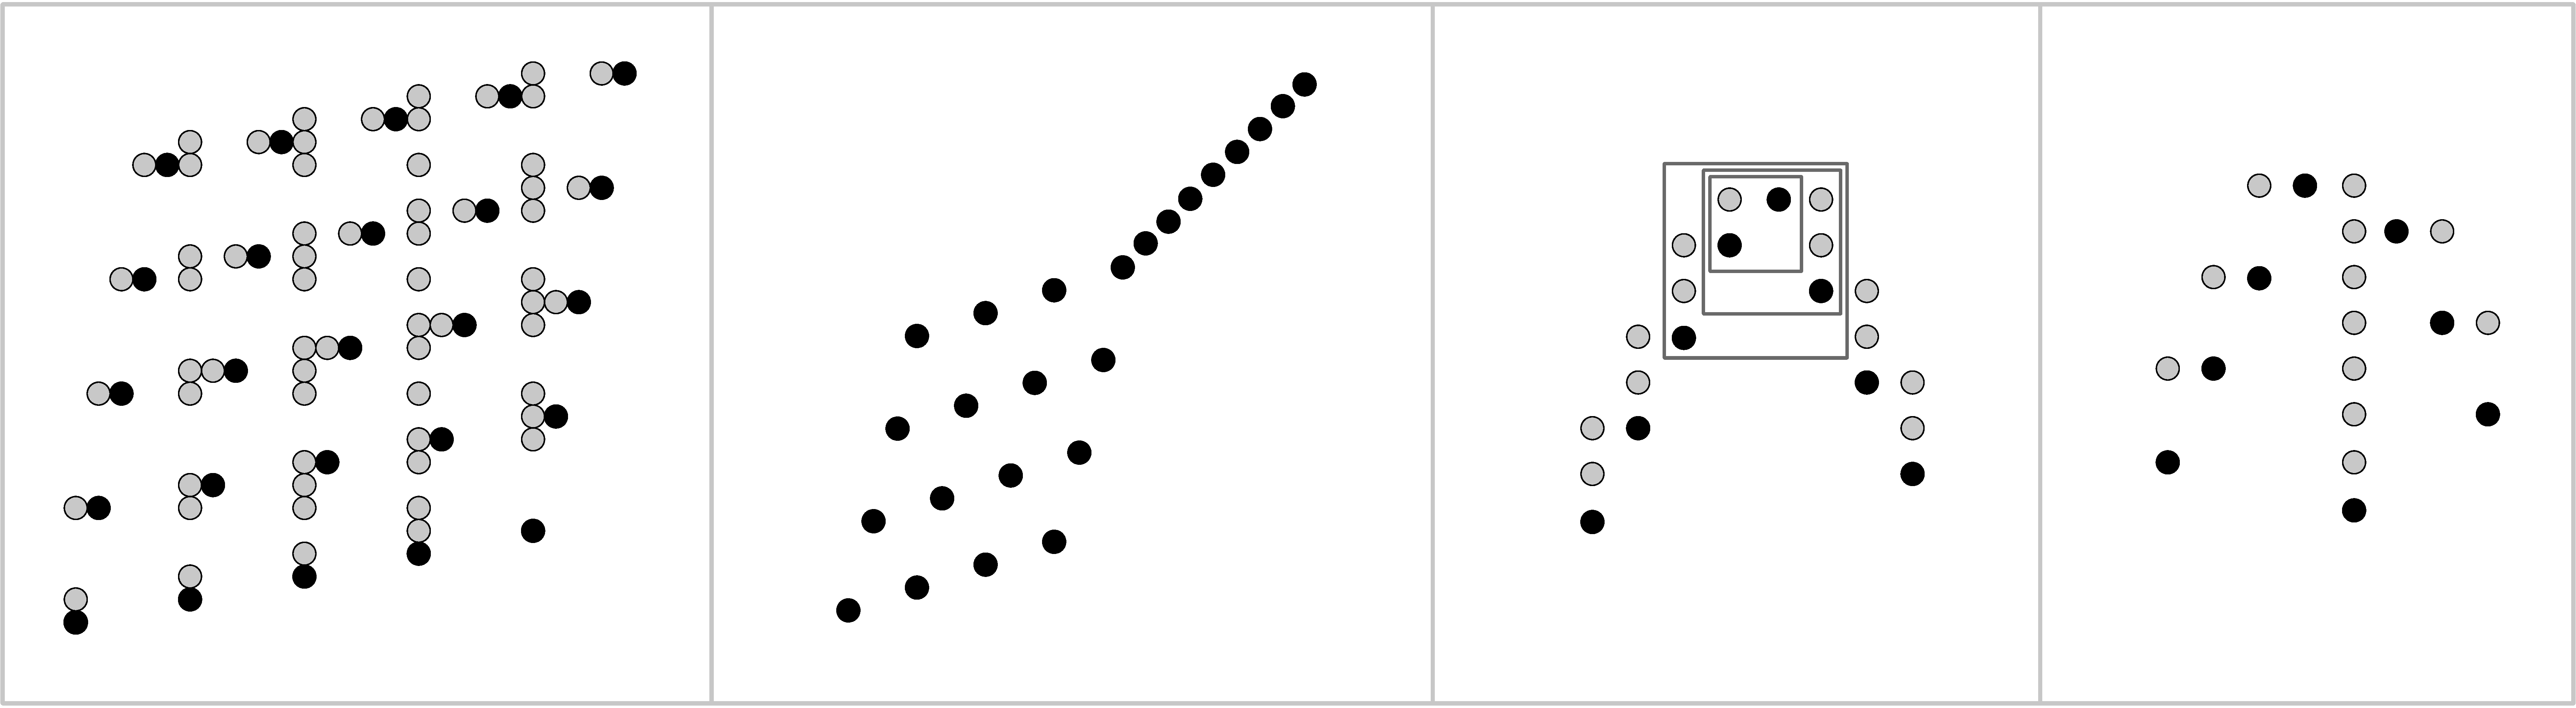
\includegraphics[scale=0.12]{examples.pdf}
\caption{From left to right: (i) ``perturbed grid'' construction when $\ell=5$ with \greedy execution, (ii) example with low dynamic finger bound, but high pattern avoidance parameter, (iii) example with low pattern avoidance parameter and high dynamic finger bound, with \greedy execution, (iv) non-decomposable permutation with linear cost \greedy execution.\label{fig:examples}} 
\end{figure}

\subsection{Why is path the roadblock to deque, traversal, split}
\label{sec:path-all}

The deque-, traversal- and split conjectures are originally stated for splay
trees. We first state the conjectures for any online BST $\cA$.
\begin{conjecture}
	[Deque conjecture \cite{tarjan_sequential}]Starting with any initial tree $T$ with $n$ elements,
	the cost of $\cA$ for inserting or deleting the current minimum or maximum elements
	$m$ times is $O(m+n)$
\end{conjecture}

\begin{conjecture}
	[Traversal conjecture \cite{ST85}]Starting with any initial tree $T$ with $n$
	elements, the cost of accessing a sequence $X$ defined by the preorder
	sequence of some BST $T'$ is $O(n)$.
\end{conjecture}

\begin{conjecture}
	[Split conjecture \cite{split_Luc91}]Starting with any initial tree $T$ with $n$ elements,
	the cost of $\cA$ for splitting $T$ by any sequence of $n$ splits is $O(n)$.
	A split at element $x$ is to delete $x$ and to obtain two trees whose
	elements are smaller resp.\ larger than $x$, each subject to
	further splittings.
\end{conjecture}

Next, we state an easier conjecture which is implied by all three
conjectures.
\begin{conjecture}
	[Path conjecture]Starting with any initial tree $T$ with $n$ elements,
	the cost of $\cA$ for accessing a sequence $X$ defined by the preorder sequence
	of some BST $T'$ which is a path is $O(n)$.
\end{conjecture}

To express it in terms of pattern avoidance,
the access sequences in the path conjecture avoid both $(2,3,1)$ and
$(2,1,3)$, while the ones in traversal conjecture only avoid $(2,3,1)$. 

Intuitively, the sequence in path conjecture is a sequence that starts
from minimum or maximum and moves inwards towards the middle, for example,
$(1,2,3,4,10,9,5,6,8,7)$.

\begin{theorem}
	Let $\cA$ be an online BST.
	\begin{enumerate}[label={{(}\roman*{)}}]
\item If $\cA$ satisfies traversal conjecture, then $\cA$ satisfies path
		conjecture. 
		\item If $\cA$ satisfies deque conjecture, then there is an online BST
		$\cA'$ that satisfies path conjecture. 
		\item If $\cA$ satisfies split conjecture, then there is an online BST $\cA'$ that satisfies path conjecture.  		
		
	\end{enumerate}
\end{theorem}
\begin{proof}
		(i) This is clear from the statement.
		
	(ii) If $\cA$ satisfies deque conjecture, then $\cA$ can delete
	the current minimum or maximum element $n$ times with cost $O(n)$.
	Observe that the sequence of these deletions can be defined by a BST
	which is a path. Given $\cA$, we construct $\cA'$ that satisfies path
	conjecture. To access $x=1$ or $n$, $\cA'$ simulates $\cA$ by deleting
	$x$, but then before finishing, $\cA'$ brings $x$ back by making $x$ the root.
	
	To access other elements $x$ from the ``minimum'' (``maximum'')
	side, $\cA'$ also simulates $\cA$, but we can see that it must touch
	$x-1$ ($x+1$) as well. Again, instead of deleting $x$, $\cA'$
	makes $x$ as a root. For any time, the cost of $\cA'$ is at most the
	cost of $\cA$ plus one. 
	


(iii) Splitting is equivalent to deleting when applied to
	the minimum or maximum element. Thus, if $\cA$ satisfies split conjecture, then $\cA$ satisfies deque conjecture without inserts. We can then use the argument of (ii).
	\end{proof}
